\documentclass[a4paper,11pt]{article}
\usepackage{amsmath,amsthm,amsfonts,amssymb,amscd,amstext,vmargin,graphics,graphicx,tabularx,multicol} 
\usepackage[francais]{babel}
\usepackage[utf8]{inputenc}  
\usepackage[T1]{fontenc} 
\usepackage{pstricks-add,tikz,tkz-tab,variations}
\usepackage[autolanguage,np]{numprint} 
\usepackage{calc}

\setmarginsrb{1.5cm}{0.5cm}{1cm}{0.5cm}{0cm}{0cm}{0cm}{0cm} %Gauche, haut, droite, haut
\newcounter{numexo}
\newcommand{\exo}[1]{\stepcounter{numexo}\noindent{\bf Exercice~\thenumexo} : }
\reversemarginpar

\newcommand{\bmul}[1]{\begin{multicols}{#1}}
\newcommand{\emul}{\end{multicols}}

\newcounter{enumtabi}
\newcounter{enumtaba}
\newcommand{\q}{\stepcounter{enumtabi} \theenumtabi.  }
\newcommand{\qa}{\stepcounter{enumtaba} (\alph{enumtaba}) }
\newcommand{\initq}{\setcounter{enumtabi}{0}}
\newcommand{\initqa}{\setcounter{enumtaba}{0}}

\newcommand{\be}{\begin{enumerate}}
\newcommand{\ee}{\end{enumerate}}
\newcommand{\bi}{\begin{itemize}}
\newcommand{\ei}{\end{itemize}}
\newcommand{\bp}{\begin{pspicture*}}
\newcommand{\ep}{\end{pspicture*}}
\newcommand{\bt}{\begin{tabular}}
\newcommand{\et}{\end{tabular}}
\renewcommand{\tabularxcolumn}[1]{>{\centering}m{#1}} %(colonne m{} centrée, au lieu de p par défault) 
\newcommand{\tnl}{\tabularnewline}

\newcommand{\trait}{\noindent \rule{\linewidth}{0.2mm}}
\newcommand{\hs}[1]{\hspace{#1}}
\newcommand{\vs}[1]{\vspace{#1}}

\newcommand{\N}{\mathbb{N}}
\newcommand{\Z}{\mathbb{Z}}
\newcommand{\R}{\mathbb{R}}
\newcommand{\C}{\mathbb{C}}
\newcommand{\Dcal}{\mathcal{D}}
\newcommand{\Ccal}{\mathcal{C}}
\newcommand{\mc}{\mathcal}

\newcommand{\vect}[1]{\overrightarrow{#1}}
\newcommand{\ds}{\displaystyle}
\newcommand{\eq}{\quad \Leftrightarrow \quad}
\newcommand{\vecti}{\vec{\imath}}
\newcommand{\vectj}{\vec{\jmath}}
\newcommand{\Oij}{(O;\vec{\imath}, \vec{\jmath})}
\newcommand{\OIJ}{(O;I,J)}


\newcommand{\reponse}[1][1]{%
\multido{}{#1}{\makebox[\linewidth]{\rule[0pt]{0pt}{20pt}\dotfill}
}}

\newcommand{\titre}[5] 
% #1: titre #2: haut gauche #3: bas gauche #4: haut droite #5: bas droite
{
\noindent #2 \hfill #4 \\
#3 \hfill #5

\vspace{-1.6cm}

\begin{center}\rule{6cm}{0.5mm}\end{center}
\vspace{0.2cm}
\begin{center}{\large{\textbf{#1}}}\end{center}
\begin{center}\rule{6cm}{0.5mm}\end{center}
}



\begin{document}
\pagestyle{empty}
\titre{Séance d'AP 1 : les puissances}{}{}{3ème}{}

\vspace*{0.2cm}

\setlength{\fboxrule}{2pt}
\begin{flushleft}
\framebox{\begin{minipage}{\linewidth}

\vspace*{0.2cm}

\underline{\textbf{Rappels de cours}}\\

Définitions : \hspace*{1cm} $a^{n} = \underbrace{a \times ... \times a}_{n fois}$  \hspace*{1.5cm}  $a^{-n} = \dfrac{1}{\underbrace{a \times ... \times a}_{n fois}}$ \\

Remarques : \hspace*{1cm}  $a^{1} = a$ \hspace*{1.5cm} $a^{0} = 1$\\

Propriétés : \hspace*{0.2cm}  $a^{n} \times a^{m} =a^{n+m}$ \hspace*{0.5cm} $\dfrac{a^{n}}{a^{m}}=a^{n-m}$ \hspace*{0.5cm} $ (a^{n})^{m} = a^{n\times m}$ \hspace*{1cm} $a^{n}\times b^{n} = (a\times b)^{n} $ \hspace*{0.5cm} $\dfrac{a^{m}}{b^{m}} = \left(\dfrac{a}{b} \right)^{m}$\\



\vspace*{0.2cm}
\end{minipage}}
\end{flushleft}

\vspace*{0.4cm}


\exo \\
Sept  voitures  transportent  chacune  sept  personnes  qui  possèdent  chacune  un  sac  avec  sept  poches.  Dans chaque poche se trouve sept enveloppes contenant chacune sept photographies.\\
Quel est le nombre total de photographies transportées ? Donner le résultat sans effectuer de calculs.\\
\reponse[2]\\

\vspace*{0.2cm}


\exo\\
Calculer les puissances suivantes en écrivant \textbf{vos étapes de calculs}.

\bmul{2}

$2^{5} = $ . . . . . . . . . . . . . . . . . . . . . . . . . . . . . . \\

$-4^{2} = $ . . . . . . . . . . . . . . . . . . . . . . . . . . . .\\


$5^{3} = $. . . . . . . . . . . . . . . . . . . . . . . . . . . . . .\\

$2^{-4} = $. . . . . . . . . . . . . . . . . . . . . . . . . . . . . .\\




\columnbreak

$(-4)^{2}= $ \reponse[1]\\

$10^{7}= $ \reponse[1]\\

$(-3)^{5} = $ \reponse[1]\\

$10^{-2} = $ \reponse[1]\\

\emul


\exo\\
En utilisant les propriétés des puissances, écrire chaque nombre sous la forme d'une seule puissance $a^{n}$

\bmul{2}

$3^{5} \times 3^{4} = $ . . . . . . . . . . . . . . . . . . . . . . . . . . . . . . \\

$ \dfrac{7^{9}}{7^{5}}= $ . . . . . . . . . . . . . . . . . . . . . . . . . . . .\\


$\dfrac{(-11)^{-3}}{(-11)^{5}} = $. . . . . . . . . . . . . . . . . . . . . . . . . . . . . .\\

$(5^{3})^{4} = $. . . . . . . . . . . . . . . . . . . . . . . . . . . . . .\\




\columnbreak

$6^{8} \times 6^{-5} = $ \reponse[1]\\

$10^{3} \times 10^{-10}= $ \reponse[1]\\

$\dfrac{4^{5}}{4^{-8}}= $ \reponse[1]\\

$9^{7} \times 2^{7} = $ \reponse[1]\\

\emul

\newpage

\exo \\
Effectuer les calculs suivants tout en détaillant vos réponses.\\

\bmul{2}

$Z =  5 - 3 \times 2^{3}$\\
\reponse[4]\\

$L =  3 \times 2^{2}  + 4 \times 5^{2}  - 3^{2}  \times 2^{3} $\\
\reponse[6]\\

$H = \dfrac{16}{(3-1)^{2}} $\\
\reponse[6]\\

\columnbreak

$ K= 2 \times (5 + 4)^{2}$\\
\reponse[4]\\

$E =  [2 + (-2)^{4}  \times 3] \times (3 ^{3} - 1)$\\
\reponse[6]\\

$D = \dfrac{(5 - 2 \times 3)^{4}}{(2-3)^{5}} $\\
\reponse[6]\\
\emul

\includegraphics[scale=0.9]{labyrinthepuissancecalcul.eps} 


\end{document}
